\appendix
\chapter{Ethics}

The following section is based on the ethics checklist provided by the Computing Department. 
The checklist consists of a series of yes/no questions. 
If an answer was yes, there is an ethical issue that needs to be considered.
These answers will form a basis for the discussion in this chapter. \\


\emph{"Does the project involve human participants?"}
The project will involve human participants in two ways: 

    - For result validation. Some results obtained in the project have been obtained with human participants, e.g. generated explanation correctness.
    
    - For dataset construction. The datasets used for this project, MLB-V2E \cite{RefWorks:RefID:16-2021automatic} and MSR-V2E \cite{RefWorks:RefID:16-2021automatic}, used human-generated explanations.

Both cases are not harmful to anyone involved. The only care that needs to be taken is regarding the personal information of the subjects involved, which is discussed in the following question.
Additionally, the participants involved in the dataset construction were compensated 15\$ per hour, as discussed in the paper under review \cite{RefWorks:RefID:16-2021automatic}.\\

\emph{"Does your project involve personal data collection and/or processing?"}

The dataset construction required subjects to explain a video in their own words.
But, this data is entirely anonymous and cannot be de-anonymised.
No explanation that is provided is in any way, shape or form personally identifiable information so that it can be linked back to a specific person.

Any data acquired from new participants during this project will be fully anonymised as well. \\

\emph{Will your project use or produce software for which there is a copyrighting licensing implication?}
The project uses three different, third-party pieces of software.
These are \emph{spacy} \cite{RefWorks:RefID:24-spacy}, \emph{FastLAS} \cite{RefWorks:RefID:19-law2020fastlas:}, \emph{ILASP} \cite{RefWorks:RefID:18-law2020ilasp}, and \emph{clingo} \cite{RefWorks:RefID:22-clingo}.
\emph{FastLAS}, \emph{spacy} and \emph{clingo} use the MIT License \cite{RefWorks:RefID:53-mit}.
The MIT License is a permissive license that does not block any future publication and only requires the preservation of copyright and license notices.
On the other hand, \emph{ILASP} is free for use for university research, but it will require reaching out to Mark Law for commercial purposes \cite{RefWorks:RefID:54-ilasp}.
The licenses are not an issue as it stands. \\


To sum up, this project has no outstanding ethical issues which need to be resolved.

\chapter{Concept Bottleneck Model}
\label{concept-bottleneck-architectures}

This appendix presents networks used in Chapter \ref{concept-bottleneck-pipeline}.
In order to reproduce the results similar to this project, one needs to train them for 100 epochs, using the adam optimiser, and the batch size of 32. \\
The number next to layer name, such as \verb_5 Dense_, represents the number of outputs of that layer.
The network for the MLB-V2E dataset is shown in \ref{mlb-network-1} and \ref{mlb-network-2}, while the bird-flowers datset network is in \ref{birds-flowers-network}.

\begin{figure}[h]
\caption{MLB-V2E baseball network part 1}
\vspace{10pt}
\centering
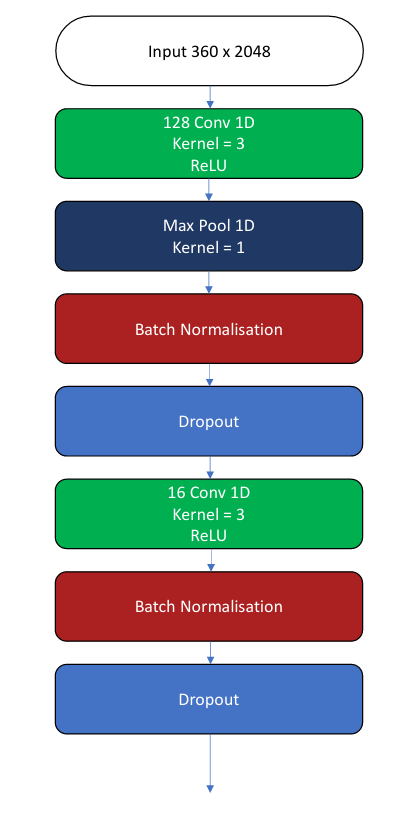
\includegraphics[width=0.6\textwidth]{appendix/mlb-network part 1.png}
\label{mlb-network-1}
\end{figure}

\begin{figure}[h]
\caption{MLB-V2E baseball network part 1}
\vspace{10pt}
\centering
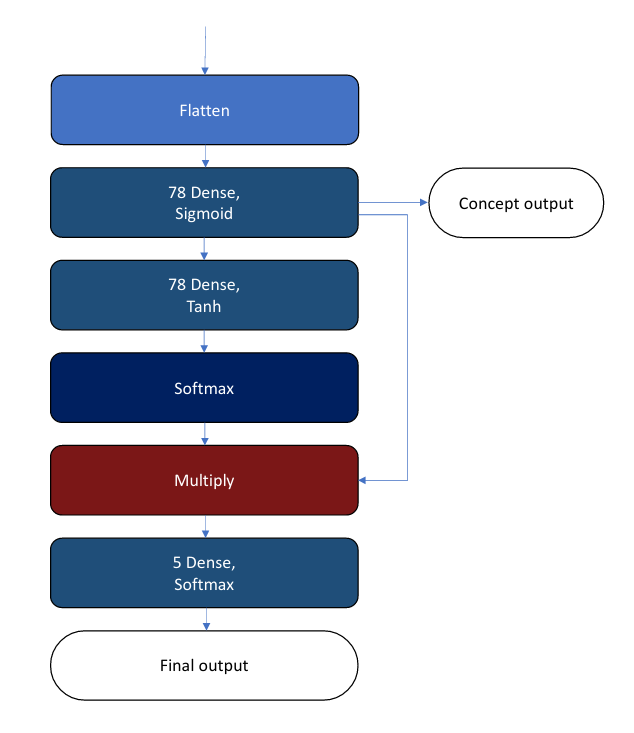
\includegraphics[width=\textwidth]{appendix/mlb network part 2.png}
\label{mlb-network-2}
\end{figure}

\begin{figure}[h]
\caption{MLB-V2E baseball network part 1}
\vspace{10pt}
\centering
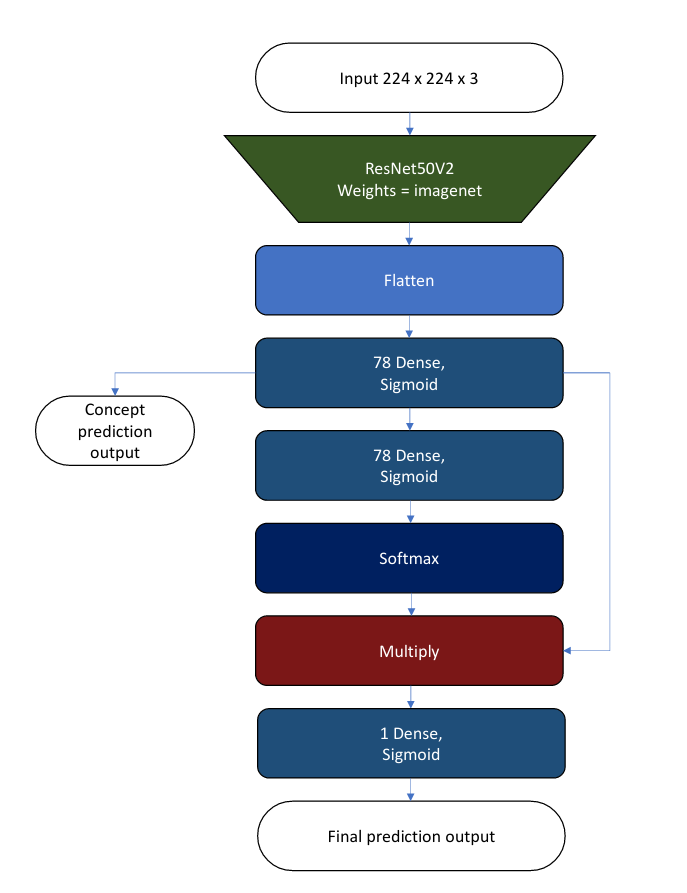
\includegraphics[width=\textwidth]{appendix/birds flowers prediction network.png}
\label{birds-flowers-network}
\end{figure}

\chapter{PyLASP scripts}
\label{pylasp-scripts-appendix}

We show the PyLASP scripts used for running the learning tasks.
Atomisation:
\begin{lstlisting}
#ilasp_script
import time

ilasp.cdilp.initialise()
solve_result = ilasp.cdilp.solve()

ilasp.stats.print_new_iteration()
debug_print('Searching for counterexample...')

c_egs = None
if solve_result is not None:
  c_egs = ilasp.find_all_counterexamples(solve_result)

conflict_analysis_strategy = {
  'positive-strategy': 'single-ufs',
  'negative-strategy': 'single-as',
  'brave-strategy':    'single-ufs',
  'cautious-strategy': 'single-as-pair'
}

start_time = time.time()
max_time = 15 * 60 * 60 # 15 hours
best_solve_result = solve_result
best_score = sum(list(map(lambda x: x['penalty'], c_egs)))

print(solve_result)

while c_egs and solve_result is not None and (time.time() - start_time) < max_time:
    
  ce = ilasp.get_example(c_egs[0]['id'])
  debug_print('Found', ce['type'], 'counterexample:', ce['id'], '(a total of', len(c_egs), 'counterexamples found)')

  constraint = ilasp.cdilp.analyse_conflict(solve_result['hypothesis'], ce['id'], conflict_analysis_strategy)

  # An example with recorded penalty of 0 is in reality an example with an
  # infinite penalty, meaning that it must be covered. Constraint propagation is,
  # therefore, unnecessary.
  if not ce['penalty'] == 0:
    c_eg_ids = list(map(lambda x: x['id'], c_egs))
    debug_print('Computed constraint. Now propagating to other examples...')
    prop_egs = []
    if ce['type'] == 'positive':
      prop_egs = ilasp.cdilp.propagate_constraint(constraint, c_eg_ids, {'select-examples': ['positive'], 'strategy': 'cdpi-implies-constraint'})
    elif ce['type'] == 'negative':
      prop_egs = ilasp.cdilp.propagate_constraint(constraint, c_eg_ids, {'select-examples': ['negative'], 'strategy': 'neg-constraint-implies-cdpi'})
    elif ce['type'] == 'brave-order':
      prop_egs = ilasp.cdilp.propagate_constraint(constraint, c_eg_ids, {'select-examples': ['brave-order'],    'strategy': 'cdoe-implies-constraint'})
    else:
      prop_egs = [ce['id']]

    ilasp.cdilp.add_coverage_constraint(constraint, prop_egs)
    debug_print('Constraint propagated to:', prop_egs)

  else:
    ilasp.cdilp.add_coverage_constraint(constraint, [ce['id']])

  solve_result = ilasp.cdilp.solve()

  if solve_result is not None:
    debug_print('Found hypothesis:', solve_result['hypothesis'], solve_result['expected_score'])
    debug_print(ilasp.hypothesis_to_string(solve_result['hypothesis']))
    
    print("", flush=True)

    ilasp.stats.print_new_iteration()
    debug_print('Searching for counterexample...')

    c_egs = ilasp.find_all_counterexamples(solve_result)
    score = solve_result['expected_score'] + sum(list(map(lambda x: x['penalty'], c_egs)))
    debug_print("Previous hypothesis score: ", score)
    if best_score == -1 or best_score > score:
      best_score = score
      best_solve_result = solve_result
      debug_print("Best hypotesis so far found")


if solve_result:
  debug_print('\n\nFinal Hypothesis:\n\n')
  print(ilasp.hypothesis_to_string(best_solve_result['hypothesis']))
else:
  print('UNSATISFIABLE')

ilasp.stats.print_timings()

#end.

\end{lstlisting}

Generalisation:
\begin{lstlisting}
#ilasp_script
import time

ilasp.cdilp.initialise()
solve_result = ilasp.cdilp.solve()

ilasp.stats.print_new_iteration()
debug_print('Searching for counterexample...')

c_egs = None
if solve_result is not None:
  c_egs = ilasp.find_all_counterexamples(solve_result)

conflict_analysis_strategy = {
  'positive-strategy': 'single-ufs',
  'negative-strategy': 'single-as',
  'brave-strategy':    'single-ufs',
  'cautious-strategy': 'single-as-pair'
}

start_time = time.time()
max_time = 12 * 60 * 60 # 12 hours
best_solve_result = solve_result
best_score = sum(list(map(lambda x: x['penalty'], c_egs)))

while c_egs and solve_result is not None and (time.time() - start_time) < max_time:
  ce = ilasp.get_example(c_egs[0]['id'])
  debug_print('Found', ce['type'], 'counterexample:', ce['id'], '(a total of', len(c_egs), 'counterexamples found)')

  constraint = ilasp.cdilp.analyse_conflict(solve_result['hypothesis'], ce['id'], conflict_analysis_strategy)

  # An example with recorded penalty of 0 is in reality an example with an
  # infinite penalty, meaning that it must be covered. Constraint propagation is,
  # therefore, unnecessary.
  if not ce['penalty'] == 0:
    c_eg_ids = list(map(lambda x: x['id'], c_egs))
    debug_print('Computed constraint. Now propagating to other examples...')
    prop_egs = []
    if ce['type'] == 'positive':
      prop_egs = ilasp.cdilp.propagate_constraint(constraint, c_eg_ids, {'select-examples': ['positive'], 'strategy': 'cdpi-implies-constraint'})
    elif ce['type'] == 'negative':
      prop_egs = ilasp.cdilp.propagate_constraint(constraint, c_eg_ids, {'select-examples': ['negative'], 'strategy': 'neg-constraint-implies-cdpi'})
    elif ce['type'] == 'brave-order':
      prop_egs = ilasp.cdilp.propagate_constraint(constraint, c_eg_ids, {'select-examples': ['brave-order'],    'strategy': 'cdoe-implies-constraint'})
    else:
      prop_egs = [ce['id']]

    ilasp.cdilp.add_coverage_constraint(constraint, prop_egs)
    debug_print('Constraint propagated to:', prop_egs)

  else:
    ilasp.cdilp.add_coverage_constraint(constraint, [ce['id']])

  solve_result = ilasp.cdilp.solve()

  if solve_result is not None:
    debug_print('Found hypothesis:', solve_result['hypothesis'], solve_result['expected_score'])
    debug_print(ilasp.hypothesis_to_string(solve_result['hypothesis']))
    print("", flush=True, end="")
    ilasp.stats.print_new_iteration()
    debug_print('Searching for counterexample...')

    c_egs = ilasp.find_all_counterexamples(solve_result)
    score = solve_result['expected_score'] + sum(list(map(lambda x: x['penalty'], c_egs)))
    if best_score == -1 or best_score > score:
      best_score = score
      best_solve_result = solve_result


if best_solve_result:
  debug_print('\n\nFinal Hypothesis:\n\n')
  print(ilasp.hypothesis_to_string(best_solve_result['hypothesis']))
else:
  print('UNSATISFIABLE')

ilasp.stats.print_timings()

#end.


\end{lstlisting}


\chapter{Sample ILASP Learned Hypothesis}
\label{learned-solution-example-appendix}

\begin{lstlisting}
 :- dep(relcl, V1, V2).
 :- dep(acl, V1, V2).
in_generalised_sent(V1) :- dep(dobj, V2, V1).
in_generalised_sent(V1) :- dep(attr, V2, V1).
in_generalised_sent(V1) :- dep(nsubj, V2, V1).
in_generalised_sent(V1) :- dep(nsubj, V1, V2).
in_generalised_sent(V1) :- dep(neg, V2, V1).
in_generalised_sent(V1) :- dep(oprd, V2, V1).
in_generalised_sent(V1) :- dep(nsubjpass, V2, V1).
in_generalised_sent(V1) :- dep(nsubjpass, V1, V2).
in_generalised_sent(V1) :- dep(mark, V2, V1).
in_generalised_sent(V1) :- dep(prt, V2, V1).
in_generalised_sent(V1) :- in_generalised_sent(V2); dep(det, V2, V1).
in_generalised_sent(V1) :- in_generalised_sent(V2); dep(prep, V1, V2).
in_generalised_sent(V1) :- in_generalised_sent(V2); dep(pobj, V1, V2).
0 {in_generalised_sent(V1) } 1 :- dep(pobj, V2, V1).
in_generalised_sent(V1) :- in_generalised_sent(V2); dep(advmod, V2, V1).
in_generalised_sent(V1) :- in_generalised_sent(V2); dep(aux, V2, V1).
in_generalised_sent(V1) :- in_generalised_sent(V2); dep(case, V2, V1).
in_generalised_sent(V1) :- in_generalised_sent(V2); dep(auxpass, V2, V1).
in_generalised_sent(V1) :- in_generalised_sent(V2); dep(compound, V2, V1).
0 {in_generalised_sent(V1) } 1 :- in_generalised_sent(V2); dep(amod, V2, V1).
0 {in_generalised_sent(V1) } 1 :- in_generalised_sent(V2); dep(poss, V2, V1).
\end{lstlisting}